% @author Benjamin Schröder
%
\chapter{Auswertung}
\label{chap:auswertung}
Werten wir die vorgestellte Implementierung nun aus. Dazu überprüfen wir zunächst die anfangs vorgestellten Anforderungen an die gesamte
Software und diskutieren anschließend, wie erfolgreich dabei das eigentliche Verfahren umgesetzt wurde. Dazu werden einige
Beispieldurchläufe mit verschiedenen Parameter-Konfigurationen betrachtet.

\section{Überprüfen der Anforderungen}
\subsection{Funktionale Anforderungen}
\subsubsection{Funktionale Anforderung 1}
\textit{Es sollen beliebige polygonale 2D-Strukturen als Input eingelesen werden können.} Diese Anforderung wird
durch die entwickelte \code{PolygonMesh} Datenstruktur realisiert. In dieser können beliebige Polygone in eine größere zusammenhängende
Struktur gebracht werden. Diese Datenstruktur kann von der \code{GrammarBuilder} Klasse als Input entgegengenommen werden, was die
Grundlage für das Durchführen aller weiteren Teilschritte des Verfahrens darstellt.

\subsubsection{Funktionale Anforderung 2}
\textit{Es sollen einige Beispielstrukturen als Input zur Verfügung gestellt werden, zwischen denen der Nutzer auswählen kann.}
Dies wird durch die vorgestellte \code{InputScene} realisiert. Hier kann der Benutzer ein Dropdown-Menü öffnen und erhält eine Liste an
möglichen Beispielstrukturen, die alle vom \code{InversePcgController} in ein \code{PolygonMesh} Objekt umgewandelt werden können.
Beispielstrukturen können ohne viel Aufwand und ohne Anpassung des Codes entfernt, hinzugefügt oder ausgetauscht werden, da diese in
separaten \code{.mesh}-Dateien gespeichert werden und dynamisch zur Laufzeit eingelesen werden können.

\subsubsection{Funktionale Anforderung 3}
\textit{Es sollen automatisch zum Input lokal ähnliche Strukturen generiert werden können.} Die Theorie hinter dem implementierten Verfahren beruht
vollständig auf den in \autoref{chap:konzept} vorgestellten Konzepten und erzeugt den Output nach dem dort beschriebenen Vorgehen. Ist das Verfahren
erfolgreich durchgelaufen, so lässt sich jeder Teil der dadurch erzeugten Outputstruktur im Input wiederfinden und die erzeugte Strukture ist somit
lokal ähnlich zum Input. In vielen Fällen kann das Verfahren aufgrund von Defiziten in der \code{MeshSolver} Komponente jedoch nicht erfolgreich durchlaufen,
wodurch diese Anforderung nicht immer vollständig erfüllt werden kann.

\textit{a) Aus einer eingelesenen Inputstruktur sollen automatisch Regeln für eine Graphgrammatik abgeleitet werden können.} Diese Anforderung wird
durch die Klasse \code{GrammarBuilder} realisiert, welche ein gegebenes \code{PolygonMesh} Objekt in eine \code{GraphGrammar} umwandeln kann.

\textit{b) Aus einer gegebenen Graphgrammatik sollen verschiedene Graphen abgeleitet werden können.} Hierfür ist die \code{GraphBuilder} Klasse zuständig.
Der dort entwickelte Algorithmus nimmt ein \code{GraphGrammar} Objekt entgegen und erzeugt daraus ein neues \code{AngleGraph} Objekt.

\textit{c) Aus einem solchen Graphen soll dann eine planare Outputstruktur mit fester Geometrie (also festen Knotenpositionen) erzeugt werden können.}
Dies wird vom \code{MeshSolver} übernommen, welcher ein \code{AngleGraph} Objekt in ein \code{PolygonMesh} Objekt umwandeln kann. Hier gibt es allerdings
das Problem, dass in vielen Fällen keine valide Lösung für die Outputstruktur gefunden werden kann. Bei der Verarbeitung etwas größerer Winkelgraphen
entstehen beim Lösen des entstandenen Gleichungssystems so viele freie Variablen, dass es eine ziemlich große Wahrscheinlichkeit gibt, dass zumindest
eine dieser Variablen zum Erzeugen von ungültigen Werten für eine der anderen unbekannten Variablen führt. Dies versuchen wir zu umgehen, indem
dieser Vorgang bis zu \code{maxTries} Mal wiederholt wird, in der Hoffnung, dass die jeweils nächste zufällige Lösung gültig sein wird. Da jedes Mal
jedoch alle Variablen erneut generiert werden, ist die Fehlerwahrscheinlichkeit dabei so hoch, dass in den meisten Fällen auch nach etlichen Versuchen
keine valide Lösung generiert werden kann. In diesem Fall visualisieren wir trotzdem die zuletzt erzeugte Struktur, jedoch wird diese nicht vollständig
zum Input lokal ähnlich sein.

\subsubsection{Funktionale Anforderung 4}
\textit{Es soll eine grafische Benutzeroberfläche geben, in welcher der Nutzer Parameter für die Generierung einstellen, sowie zwischen
den verschiedenen Inputstrukturen auswählen können soll.} Dies wird durch die Klasse \code{InversePcgApplication} realisiert. In den drei darin
implementierten Szenen kann der Nutzer alle wichtigen Einstellungen vornehmen. In der \code{InputScene} kann der Seed für den Zufallsgenerator festgelegt
und eine Inputstruktur ausgewählt werden. In der \code{GrammarScene} kann die Anzahl an Generation in der Graph-Hierarchie festgelegt werden. In der
\code{OutputScene} können alle weiteren in \autoref{chap:datenmodell} vorgestellten Parameter eingestellt werden.

\subsubsection{Funktionale Anforderung 5}
\textit{Sowohl die Inputstrukturen, die daraus erzeugt Grammatik und die generierten Variationen sollen visualisiert werden können.} Die Visualisierung
der hier genannten Datenstrukturen wird ebenfalls durch die \code{InversePcgApplication} übernommen. In der \code{InputScene} wird die ausgewählte
Inputstruktur dargestellt, die \code{GrammarScene} übernimmt das Darstellen der daraus erzeugten Grammatik, und die \code{OutputScene} wird zum
Visualisieren der verschiedenen erzeugten Variationen benutzt.

\subsection{Nichtfunktionale Anforderungen}
\subsubsection{Nichtfunktionale Anforderung 1}
\textit{Die Anwendung soll auf Windows ausführbar sein.} Der gesamte Code wurde auf einem Windows 11 PC und einem Laptop mit Windows 10 implementiert
und getestet. Bei der Ausführung der Anwendung auf beiden Geräten gibt es keine Probleme. Die Anforderung wurde also erfüllt.

\subsubsection{Nichtfunktionale Anforderung 2}
\textit{Die Nutzeroberfläche soll einfach und übersichtlich gehalten werden.} Die implementierte Benutzeroberfläche wurde sehr simpel gestaltet und
stellt nur die wichtigsten Funktionen bereit. Es gibt lediglich drei verschiedene Szenen, welche jeweils nur aus einem Viewport und einer kurzen
Reihe an Einstellungsmöglichkeiten, sowie einem Knopf zum Senden eines Befehls an die Steuerungskomponente bestehen. Alles wird in einem Fenster
dargestellt, es gibt keine Pop-ups und mit der Ausnahme des Dropdown-Menüs zum Auswählen der Inputstruktur auch keine aufklappbaren Komponenten mit
versteckter Komplexität. Da die Anwendung vollständig mit Swing und AWT umgesetzt wurde, ist das Design der verwendeten GUI-Komponenten selbst ebenfalls
sehr simpel gehalten.

\subsubsection{Nichtfunktionale Anforderung 3}
\textit{Die implementierten Algorithmen sollen sich deterministisch verhalten und alle Ergebnisse sollen reproduzierbar sein.} Auch diese Anforderung
wird erfüllt. Alle Algorithmen, bei denen das Erzeugen von Zufallszahlen eine Rolle spielt, erhalten die Zufallszahlen von ein und demselben
Zufallszahlengenerator, der von der Steuerungskomponente verwaltet wird. Dieser wird stets mit einem vom Benutzer festgelegten Seed initialisiert und
erzeugt bei gleichem Seed stets die gleichen zufälligen Zahlen. Werden vom Nutzer nach Start der Anwendung die exakt gleichen Aktionen immer und immer
wiederholt, so sind die erzeugten Ergebnisse ebenfalls immer und immer wieder identisch.

\subsubsection{Nichtfunktionale Anforderung 4}
\textit{Die Software soll modular aufgebaut sein, wobei die Module selbst eine hohe Kohäsion vorweisen und untereinander schwach gekoppelt sein sollen.}
Wie in \autoref{chap:architektur} ausführlich erklärt wurde, besteht die entwickelte Software aus vielen verschiedenen in sich logisch gekapselten Komponenten.
Aufgrund des gewählten \gls{ac:mvc}-Entwurfsmusters sind die drei Hauptkomponenten Ansicht, Datenmodell und Steuerung lose untereinander gekoppelt und können
größtenteils unabhängig voneinander existieren. \cite{48_bucanek} Es werden einheitliche Schnittstellen geboten oder die Informationen werden über das Beobachter-Muster
zwischen den Komponenten ausgetauscht. In beiden Fällen wäre ein Austauschen der einzelnen Komponenten ledglich mit sehr geringem Aufwand verbunden. Die
Kohäsion innerhalb der einzelnen Module ist hoch, da diese jeweils einen klar definierten Aufgabenbereich haben und die gesamte darin umgesetzte Funktionalität
nur zum Umsetzen der entsprechenden Aufgabe des Moduls genutzt wird. Funktionalität, die sich von mehreren Komponenten geteilt wird, wurde in eine separate
Klasse \code{Utils} ausgelagert. Die Komponenten mit der niedrigsten Kohäsion sind die Klassen \code{PolygonMesh} und \code{AngleGraph}, da diese neben dem
Definieren der entsprechenden Datenstruktur auch komplexere Funktionalität für die Transformation dieser Datenstruktur enthalten. Diese Funktionalität
hätte jeweils eventuell auch in eine separate Klasse ausgelagert werden können.

\subsubsection{Nichtfunktionale Anforderung 5}
\textit{Alle wichtigen Komponenten sollen durch Tests abgedeckt sein.} Diese Anforderung wurde größtenteils umgesetzt. Es gibt separate Testklassen für
die drei implementierten Algorithmus-Klassen \code{GrammarBuilder}, \code{GraphBuilder} und \code{MeshSolver}. In diesen wird jeweils der gesamte Ablauf
des entsprechenden implementierten Teilschritts getestet, indem die erhaltenen Endergebnisse überprüft werden. Außerdem befinden sich dort Tests für
viele, aber nicht alle, Teilfunktionen, die dabei genutzt werden. Auch für die Datenstrukturen gibt es Tests, allerdings nur für die Klassen \code{AngleGraph}
und \code{PolygonMesh}, da diese Funktionalität für komplexere Transformationen der entsprechenden Datenstrukturen enthalten.

\subsubsection{Nichtfunktionale Anforderung 6}
\textit{Der Code soll verständlich sein und alle nicht-trivialen Bestandteile des Codes sollen mit Kommentaren versehen werden.} Jede von uns selbst
implementierte und nicht von anderen Klassen geerbte Methode wurde mit Javadoc-Kommentaren versehen, die die genaue Funktionsweise, die involvierten
Paramater und den Rückgabewert der Methode erklären. Komplexere Methoden wurden außerdem intern mit weiteren Kommentaren versehen, wenn die einzelnen
Teilschritte als nicht-trivial erachtet wurden. Die Benennung der verschiedenen Klassen, Methoden und Variablen wurde so gewählt, dass diese so präzise
wie möglich den entsprechenden Zweck beschreiben. Generell wurde der Code auf Basis der in \cite{49_java_conventions} vorgestellten Konventionen erstellt.
Damit gilt diese Anforderung als erfüllt.

\section{Beispieldurchläufe}
Nachfolgend werden einige der erhaltenen Ergebnisse präsentiert, welche mithilfe von verschiedenen Parameter-Konfigurationen erzeugt wurden. Zunächst
zeigen wir einige erfolgreiche Ergebnisse. Es werden jeweils die verwendete Inputstruktur, die daraus erzeugte Grammatik, sowie die letztendliche Outputstruktur
dargestellt. Die Grammatik kann in den meisten Fällen aufgrund der großen Anzahl an Regeln nicht vollständig dargestellt werden und es wird jeweils nur ein
Ausschnitt an Regeln gezeigt. Außerdem werden die verwendeten Parameter-Konfigurationen für jedes Beispiel gezeigt.

\subsection{Erfolgreiche Durchläufe}

\subsubsection{Haus}
\begin{figure}[H]
    \centering
    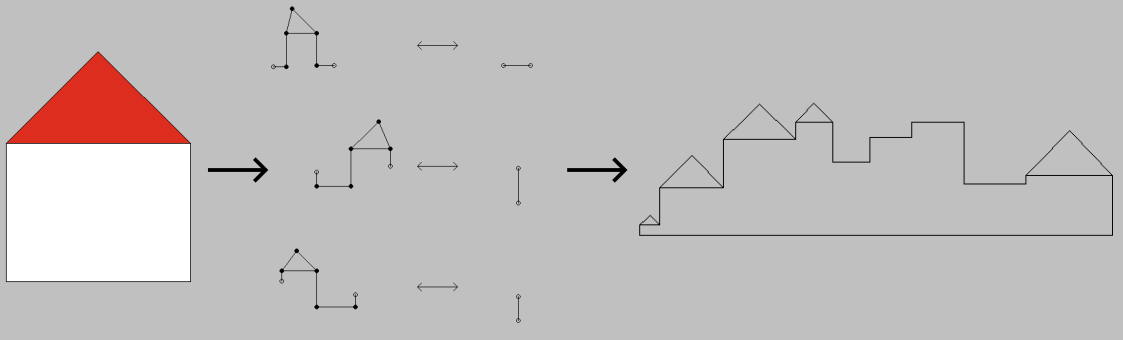
\includegraphics[width=\textwidth]{images/house_success.png}
    \caption{Erfolgreicher Durchlauf mit Input-Datei \code{house.mesh}.}
    \label{fig:house_success}
\end{figure}
Für den in Abbildung \ref{fig:house_success} dargestellten Durchlauf verwendete Parameter-Konfiguration: \code{seed = 23456}, \ \code{maxGeneration = 6}, \ \code{iterations = 5},
\ \code{maxTries = 100}, \ \code{minRandVal = 10}, \ \code{maxRandVal = 100}. Die Ergebnisse entsprechen den Erwartungen.

\subsubsection{Quadrat}
\begin{figure}[H]
    \centering
    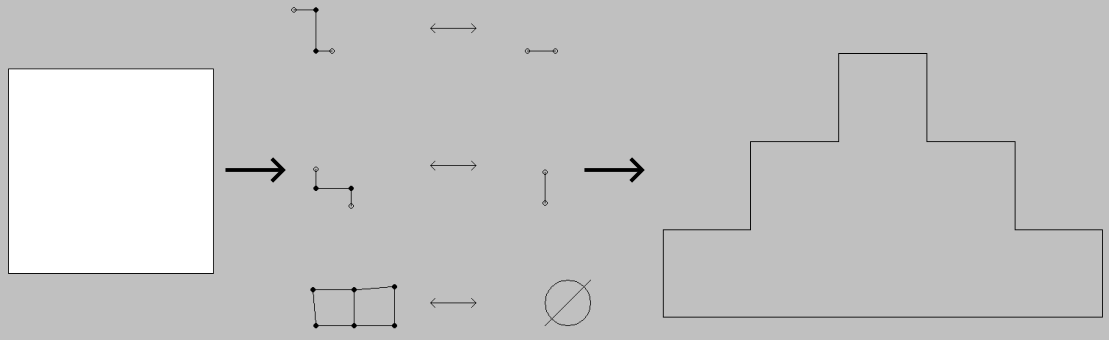
\includegraphics[width=\textwidth]{images/square_success.png}
    \caption{Erfolgreicher Durchlauf mit Input-Datei \code{square.mesh}.}
    \label{fig:square_success}
\end{figure}
Für den in Abbildung \ref{fig:square_success} dargestellten Durchlauf verwendete Parameter-Konfiguration: \code{seed = 5555}, \ \code{maxGeneration = 3}, \ \code{iterations = 5},
\ \code{maxTries = 100}, \ \code{minRandVal = 10}, \ \code{maxRandVal = 10}. Die Ergebnisse entsprechen den Erwartungen. Durch das Limitieren der Zufallszahlen auf nur
exakt einen Wert enthält der Output sehr viele Kanten mit der gleichen Kantenlänge und nimmt somit eine regelmäßige Form an. Es wirkt, als wäre der Output auf
Basis eines Gitters modelliert worden.

\subsubsection{Doppeltes Quadrat}
\begin{figure}[H]
    \centering
    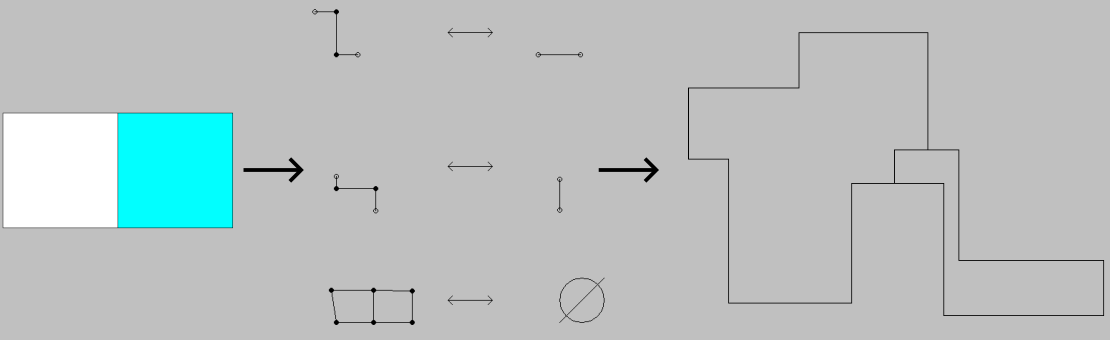
\includegraphics[width=\textwidth]{images/square_double_success.png}
    \caption{Erfolgreicher Durchlauf mit Input-Datei \code{square\_double.mesh}.}
    \label{fig:square_double_success}
\end{figure}
Für den in Abbildung \ref{fig:square_double_success} dargestellten Durchlauf verwendete Parameter-Konfiguration: \code{seed = 77}, \ \code{maxGeneration = 3}, \ \code{iterations = 7},
\ \code{maxTries = 100}, \ \code{minRandVal = 10}, \ \code{maxRandVal = 100}. Die Ergebnisse entsprechen den Erwartungen.

\subsubsection{Raute}
\begin{figure}[H]
    \centering
    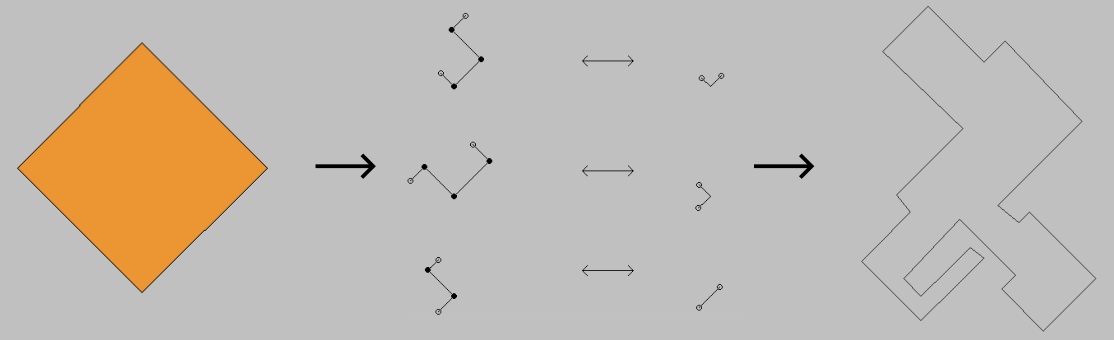
\includegraphics[width=\textwidth]{images/rhombus_success.png}
    \caption{Erfolgreicher Durchlauf mit Input-Datei \code{rhombus.mesh}.}
    \label{fig:rhombus_success}
\end{figure}
Für den in Abbildung \ref{fig:rhombus_success} dargestellten Durchlauf verwendete Parameter-Konfiguration: \code{seed = 123}, \ \code{maxGeneration = 3}, \ \code{iterations = 10},
\ \code{maxTries = 100}, \ \code{minRandVal = 10}, \ \code{maxRandVal = 70}. Die Ergebnisse entsprechen den Erwartungen.

\subsection{Fehlerhafte Durchläufe}

\subsubsection{Haus}
\begin{figure}[H]
    \centering
    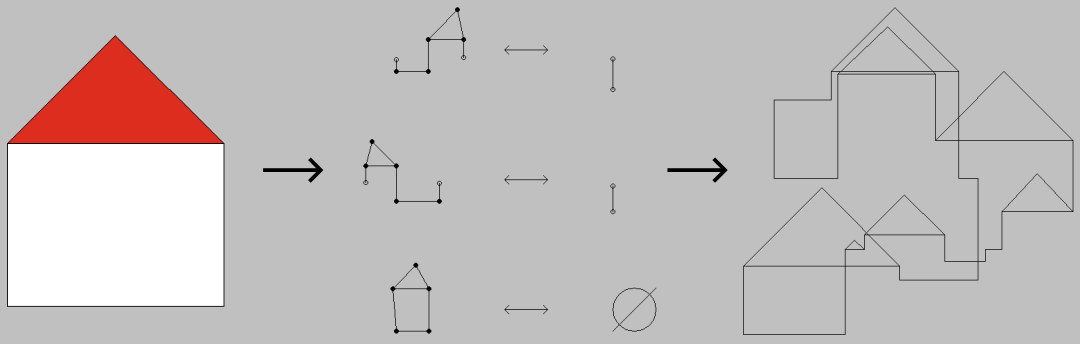
\includegraphics[width=\textwidth]{images/house_fail.png}
    \caption{Fehlerhafter Durchlauf mit Input-Datei \code{house.mesh}.}
    \label{fig:house_fail}
\end{figure}
Für den in Abbildung \ref{fig:house_fail} dargestellten Durchlauf verwendete Parameter-Konfiguration: \code{seed = 337}, \ \code{maxGeneration = 7}, \ \code{iterations = 7},
\ \code{maxTries = 100}, \ \code{minRandVal = 10}, \ \code{maxRandVal = 100}. Die Ergebnisse entsprechen nicht den Erwartungen. Alle dargestellten Kantenwinkel
lassen sich zwar im Input wiederfinden und es wirkt so, als wäre die erzeugte Outputstruktur zumindest lokal ähnlich zum Input. Das Ergebnis ist jedoch
trotzdem fehlerhaft, da sich einige der Kanten überschneiden.

\subsubsection{Achteck}
\begin{figure}[H]
    \centering
    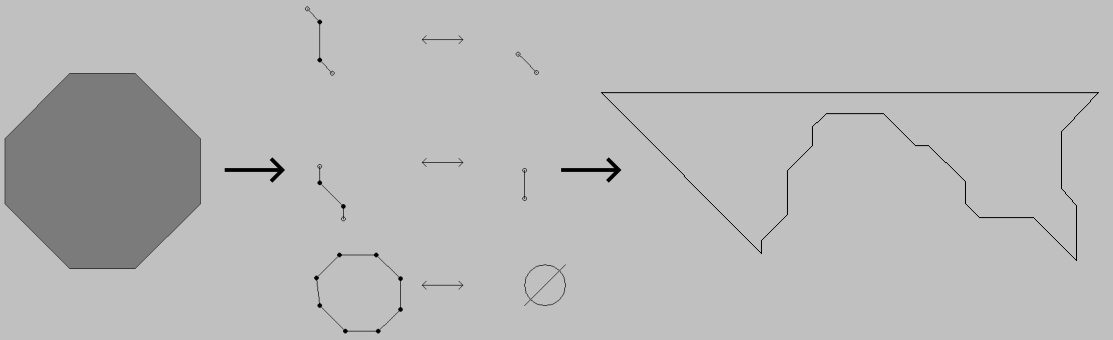
\includegraphics[width=\textwidth]{images/octagon_fail.png}
    \caption{Fehlerhafter Durchlauf mit Input-Datei \code{octagon.mesh}.}
    \label{fig:octagon_fail}
\end{figure}
Für den in Abbildung \ref{fig:octagon_fail} dargestellten Durchlauf verwendete Parameter-Konfiguration: \code{seed = 445}, \ \code{maxGeneration = 2}, \ \code{iterations = 7},
\ \code{maxTries = 10}, \ \code{minRandVal = 10}, \ \code{maxRandVal = 100}. Diesmal ist der dargestellte Output planar, jedoch liegt hier keine lokale Ähnlichkeit
vor. Die Kantenwinkel stimmen zwar alle mit den Kantenwinkeln im Input überein, jedoch unterscheidet sich die Topologie der beiden Strukturen an einigen Stellen.
Einige der Knoten in der Outputstruktur lassen sich nicht im Input wiederfinden (die ``Spitzen'').

\subsubsection{Dreieck}
\begin{figure}[H]  
    \centering  
    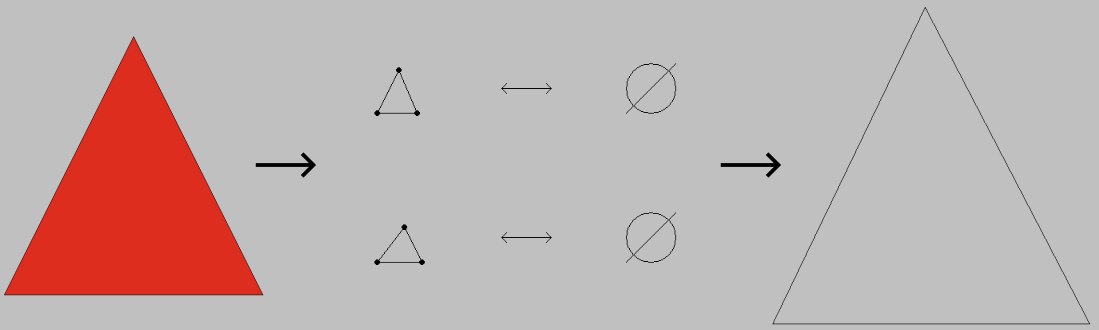
\includegraphics[width=\textwidth]{images/triangle_fail.png}
    \caption{Ungenügender Durchlauf mit Input-Datei \code{triangle.mesh}.}
    \label{fig:triangle_fail}
\end{figure}
Für den in Abbildung \ref{fig:triangle_fail} dargestellten Durchlauf verwendete Parameter-Konfiguration: \code{seed = 23456}, \ \code{maxGeneration = 30}, \ \code{iterations = 3},
\ \code{maxTries = 100}, \ \code{minRandVal = 10}, \ \code{maxRandVal = 100}. Der Output entspricht den geforderten Eigenschaften, ist sowohl zum Input lokal
ähnlich als auch planar und somit nicht fehlerhaft. Trotzdem ist das Ergebnis unbrauchbar, da sich der Output kaum vom Input unterscheidet. Der Output
besitzt zwar andere Kantenlängen, ist strukturell allerdings exakt gleich aufgebaut. Trotz der hohen Anzahl an zugelassenen Generationen konnte das Verfahren
lediglich nur eine einzige Starter-Regel für die Grammatik ableiten (beide dargestellten Starter-Regeln sind identisch). Aus dieser Grammatik kann keine
hohe Vielfalt an Ergebnissen erzeugt werden.

\section{Auswertung der Ergebnisse}
Allgemein sind die Ergebnisse durchaus zufriedenstellend. Die erzeugten Strukturen erfüllen zwar in vielen Fällen nicht die Anforderungen an die lokale
Ähnlichkeit und können auch oft nicht ohne Überschneidungen einiger der Kanten dargestellt werden, jedoch wird durch die von uns implementierte Software
klar demonstriert, dass dieses Verfahren grundsätzlich funktioniert. Auch wenn es dabei noch viele Probleme gibt, die behoben werden müssen um dieses
Verfahren wirklich in der Praxis einsetzen zu können, erfüllt die entwickelte Anwendung voll und ganz ihren Zweck als Prototyp.
